% Name: Expression tree
% Description: The expression (a + b) × c − d ÷ e as a tree, with operators at the inner nodes and operands at the leaves.
% Tags: expression tree, parse tree, arithmetic, data structure

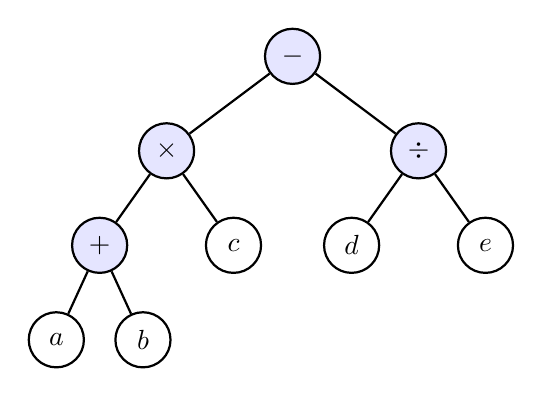
\begin{tikzpicture}[
  level distance=12mm,
  level 1/.style={sibling distance=32mm},
  level 2/.style={sibling distance=17mm},
  level 3/.style={sibling distance=11mm},
  op/.style={circle, draw, thick, fill=blue!10, minimum size=7mm, inner sep=0pt},
  var/.style={circle, draw, thick, minimum size=7mm, inner sep=0pt},
  edge from parent/.style={draw, thick},
]
  \node[op] {$-$}
    child { node[op] {$\times$}
      child { node[op] {$+$}
        child { node[var] {$a$} }
        child { node[var] {$b$} }
      }
      child { node[var] {$c$} }
    }
    child { node[op] {$\div$}
      child { node[var] {$d$} }
      child { node[var] {$e$} }
    };
\end{tikzpicture}
